%%%%%%%%%%%%%%%%%%%%%%%%%%%%%%%%%%%%%%%%%%%%%%%%%%%%
%%%% En-tête leçon
\begin{headerBlock}
  \chapter{Traitement d'un signal. Etude spectrale.}
    \label{LP_TraitementSignal}
\end{headerBlock}

%%%%%%%%%%%%%%%%%%%%%%%%%%%%%%%%%%%%%%%%%%%%%%%%%%%%
%%%% Références
\begin{center}
\begin{tabularx}{\textwidth}{| X | X | c | c |}
  \hline
  \rowcolor{gray!20}\multicolumn{4}{c}{Bibliographie de la leçon : } \\
  \hline 
  Titre & Auteurs & Editeur (année) & ISBN \\
  \hline
  Electronique & Pérez & Dunod &   \\
  \hline 
  Traitement des signaux et acquisition de données & Francis Cottet & Dunod & 2-10-006312-X \\
  \hline 
  Tout-en-un PSI &  & Tec\&Doc & \\
  \hline
  Dictionnaire de physique & R. Taillet, L. Villain, P. Febvre & de Boeck & \\
  \hline
  Cours Jérémy Neveu & J. Neveu & & \\
  \hline
\end{tabularx}
\end{center}

%%%%%%%%%%%%%%%%%%%%%%%%%%%%%%%%%%%%%%%%%%%%%%%%%%%%
\begin{reportBlock}{Plan détaillé}
  \textbf{Niveau choisi pour la leçon :} CPGE deuxième année
  \newline
  \textbf{Prérequis : }
  \begin{itemize}
      \item Electrocinétique : impédance, association série/parallèle, pont diviseur de tension 
      \item 
  \end{itemize}


\section*{Introduction}
\textcolor{red}{Accroche : (cf cours Jérémy Neveu) }L'enjeu des communications est de pouvoir envoyer un signal (\textit{i.e.} une information) depuis un émetteur jusqu'à un récepteur afin que celui-ci puisse être d'une part reçu et d'autre part compris.
\begin{center}
    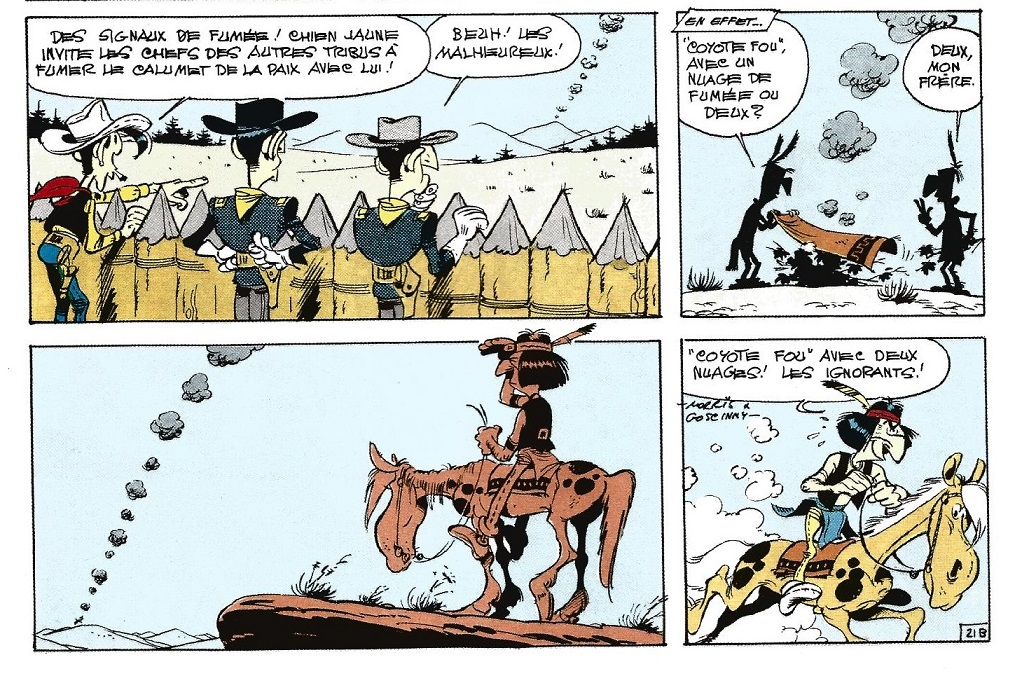
\includegraphics[scale=0.8]{LP_TraitementSignal/Codage_LuckyLuke.jpg}
\end{center}
\textcolor{green}{signal :} (ref Taillet p674) Variation temporelle ou spatiale d'une quantité physique mesurable (tension, force, lumière, ...) portant une information.\\
\textcolor{green}{Traitement du signal :} Transformation d'un signal reçu par un récepteur pour en retirer l'information transmise initialement par un émetteur. Ex : si un observateur cherche à analyser les nuages émis par le feu (\textcolor{green}{signal}), il doit se séparer de celle émise par l'environnement (\textcolor{green}{bruit}) par différents moyen (se couvrir les yeux pour se protéger du soleil). \og Se couvrir les yeux \fg~ = filtrage.

\section{Spectre et filtrage d'un signal}

\subsection{Décomposition Fourier}

Cf Cottet Chap 2 - Tout signal peut se décomposer comme une série de signaux sinusoïdaux.\\

Cf Cottet p14- Spectre d'énergie (important pour la suite car modulation DBPC problèmatique) d'un signal cf Cottet. Composante continue, fondamental, harmoniques.\\

Propriétés TF (?) et principe de la FFT sur un oscillo (pour préparer les mesures de la deuxième partie)

\subsection{Types de signaux}
Signaux analogiques vs numériques, déterministes vs aléatoires. On va se concentrer sur les signaux analogiques et déterministes.


\subsection{Réponse d'un filtre à une excitation périodique : exemple du filtre RC passe-bas}
Prendre l'exemple d'un circuit RC passe-bas (mesure sur la capa). \textcolor{blue}{Manip quantitative :} tracer le diagramme de Bode et déterminer la fréquence de coupure $f_c = \frac{1}{RC}$. Mettre en évidence le $-20\log(\omega)$. Déterminer la bande passante.

\subsection{Autres types de filtre}
\textbf{Transition :} Maintenant qu'on a décrit un signal et qu'on sait en retirer des informations, on va voir comment en envoyer un et comment le réceptionner.

\section{Modulation et démodulation en amplitude}
Fil conducteur : radio analogique. Cf cours de Jérémy.
Deux problèmes : 
\begin{itemize}
    \item \textcolor{green}{l'encombrement :} par exemple deux personnes qui parlent en même temps,
    \item dimension des antennes : longueur de l'antenne doit être de l'ordre de la longeur d'onde soit 1500km pour $f=20Hz$ et 1.5km pour $f=20000Hz$ ...
\end{itemize}

\subsection{Principe de la modulation en amplitude}
On souhaite passer à des tailles d'antennes raisonnable de l'ordre du mètre : soit $f=\frac{c}{\lambda}=30$MHz : c'est le principe de la modulation.

\textcolor{green}{Modulation :} Accrocher un signal à transmettre à une porteuse : modulation de la porteuse. Ex : pigeon voyageur (porteuse) pour faire passer une lettre (signal modulant) d'un point A à un point B\\

Pour un signal EM : 
\begin{itemize}
    \item $V_m(t)=A+B\cos(\omega_mt)$ pour la modulation (GBF Agilent à $\frac{\omega_m}{2\pi}=500$~Hz : le message à faire passer)
    \item $V_p(t) = V_0\cos(\omega_pt)$ (BGX Métrix à $\frac{\omega_p}{2\pi}=50$~kHz : le pigeon voyageur)
\end{itemize}

Faire le calcul à la sortie d'un multiplieur. Deux cas particuliers : montrer modulation DBPC ($A\neq0$) et DBPS ($A=0$).

\begin{center}
    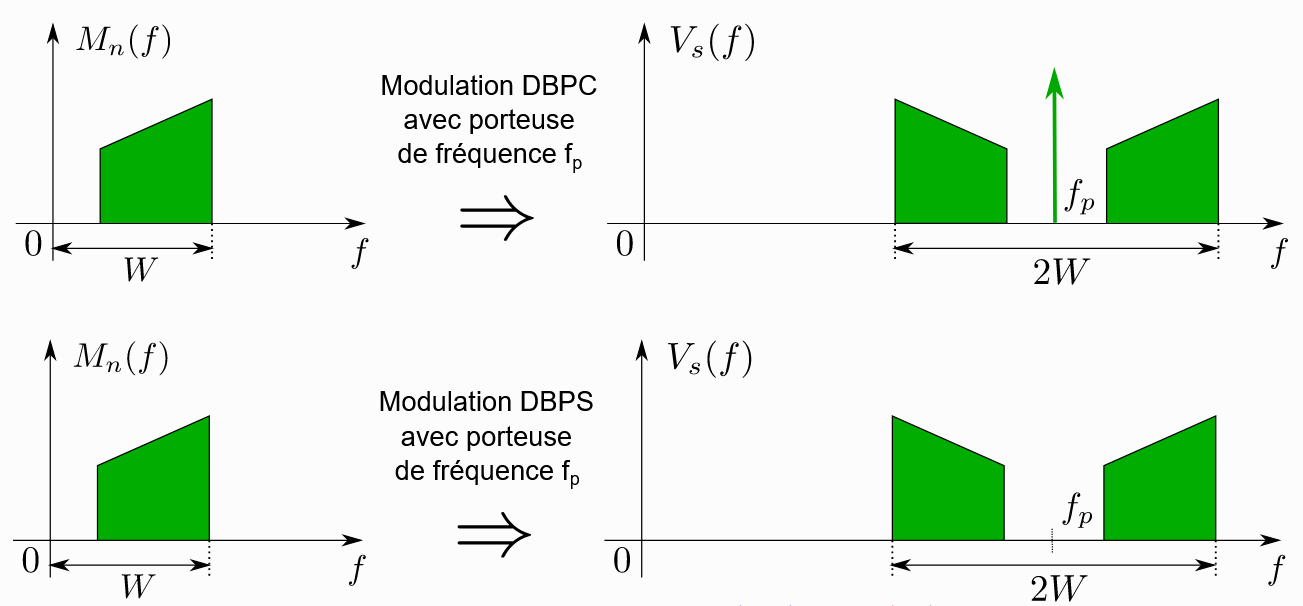
\includegraphics[scale=0.5]{LP_TraitementSignal/Modulation.png}
\end{center}



\subsection{Démodulation par détection synchrone}
Intérêt de la 
\textcolor{red}{Attention :} pour que ça puisse fonctionner, il faut que la porteuse puisse être regénérée (on peut le faire avec une boucle à vérouillage de phase cf cours Jérémy, le mentionner peut-être en conclusion de la partie).\\

\textcolor{blue}{Manip qualitative : démodulation par détection synchrone}. Le TP est bien fait, montrer le signal qu'on module, le signal après multiplication par la porteuse et le signal après le filtre passe-bas.

\textbf{Transition : }L'algorithme de FFT qu'on a largement utilisé au cours des expériences repose sur la transformée de Fourier d'un signal échantillonné (discrétisé). On va voir justement quelques avantages/inconvénients des traitements des signaux numériques.

\section{Quelques aspects du traitement des signaux numérique}

\subsection{Echantillonnage}
Voir cours de Jérémy, parler du critère de Shannon.

\subsection{Effet du fenêtrage temporel}
p190 Cottet.
\section*{Conclusion et ouverture}

Parler de la modulation en fréquence, en phase, leurs avantages. Ouvrir sur les signaux numériques. A



\end{reportBlock}